\documentclass[conference]{IEEEtran}
\IEEEoverridecommandlockouts

\usepackage[portuges]{babel}

% The preceding line is only needed to identify funding in the first footnote. If that is unneeded, please comment it out.
\usepackage{cite}
\usepackage{amsmath,amssymb,amsfonts}
\usepackage{algorithmic}
\usepackage{graphicx}
\usepackage{textcomp}
\usepackage{xcolor}

\usepackage[]{siunitx}

\bibliographystyle{IEEEtran}

% Enumerations
\usepackage[inline]{enumitem}
\renewcommand*\descriptionlabel[1]{\hspace\labelsep\itshape #1}

% Spacing
\usepackage{xspace}

% Tables
\usepackage{booktabs}
\usepackage{multirow}
\newcommand{\specialcell}[3][c]
{\begin{tabular}[#1]{@{}#2@{}}#3\end{tabular}}

% Acronyms
\usepackage[acronym,nowarn]{glossaries}
\glsdisablehyper
%==============================================================================
% Institutions 
%=============================================================================

% PUC Minas
\newacronym{pucminas}{PUC Minas}{Pontifícia Universidade Católica de Minas Gerais}
	\newcommand{\pucminas}{\gls{pucminas}\xspace}

% UFSC
\newacronym{ufsc}{UFSC}{Universidade Federal de Santa Catarina}
	\newcommand{\ufsc}{\gls{ufsc}\xspace}

% UGA
\newacronym{uga}{UGA}{Univerité Grenoble Alpes}
	\newcommand{\uga}{\gls{uga}\xspace}

% Grenoble INP
\newacronym{inpg}{Grenoble INP}{Institut National Polytechnique de Grenoble}
	\newcommand{\inpg}{\gls{inpg}\xspace}

%==============================================================================
% Computer Architecture
%=============================================================================

% Manycores
\newcommand{\scc}{Intel Single-Cloud Computer\xspace}
\newcommand{\xeonphi}{Intel Xeon Phi\xspace}
\newcommand{\tilegx}{Tilera TILE-Gx100\xspace}
\newcommand{\tilepro}{Tilera TILE64\xspace}
\newcommand{\mppa}{Kalray MPPA-256\xspace}
\newcommand{\pulp}{PULP\xspace}
\newcommand{\taihulight}{Sunway SW26010\xspace}
\newcommand{\epiphany}{Adapteva Epiphany\xspace}
\newcommand{\optimsoc}{OpTiMSoC\xspace}
\newcommand{\hero}{HERO\xspace}
\newcommand{\celerity}{Celerity\xspace}

% Architecture Families
\newcommand{\amd}{x86-64\xspace}
\newcommand{\intel}{x86\xspace}
\newcommand{\openrisc}{OpenRISC\xspace}
\newcommand{\bostan}{Bostan\xspace}
\newcommand{\riscv}{RISC-V\xspace}

% ISA
\newacronym{isa}{ISA}{Instruction Set Architecture}
	\newcommand{\isa}{\gls{isa}\xspace}

% FIFO
\newacronym{fifo}{FIFO}{First-In First-Out}
	\newcommand{\fifo}{\gls{fifo}\xspace}

% VLIW
\newacronym{vliw}{VLIW}{Very Long Instruction Word}
	\newcommand{\vliw}{\gls{vliw}\xspace}

% Taxonomy
\newacronym{mimd}{MIMD}{Multiple Instruction Multiple Data}
	\newcommand{\mimd}{\gls{mimd}\xspace}
\newacronym{simd}{SIMD}{Single Instruction Multiple Data}
	\newcommand{\simd}{\gls{simd}\xspace}
\newacronym{numa}{NUMA}{Non-Uniform Memory Access}
	\newcommand{\numa}{\gls{numa}\xspace}
\newacronym{norma}{NoRMA}{No Remote Memory Access}
	\newcommand{\norma}{\gls{norma}\xspace}
\newacronym{amp}{AMP}{Asymmetric Multi-Processing}
	\newcommand{\amp}{\gls{amp}\xspace}
\newacronym{smp}{SMP}{Symmetric Multi-Processing}
	\newcommand{\smp}{\gls{smp}\xspace}
\newacronym{gpu}{GPU}{Graphics Processing Unit}
	\newcommand{\gpu}{\gls{gpu}\xspace}
	\newcommand{\gpus}{\glspl{gpu}\xspace}
\newacronym{fpga}{FPGA}{Field Programmable Gate Array}
	\newcommand{\fpga}{\gls{fpga}\xspace}
	\newcommand{\fpgas}{\glspl{fpga}\xspace}

% Core
\newacronym{pe}{PE}{Processing Element}
	\newcommand{\pe}{\gls{pe}\xspace}
	\newcommand{\pes}{\glspl{pe}\xspace}
\newacronym{rm}{RM}{Resource Manager}
	\newcommand{\rman}{\gls{rm}\xspace}
	\newcommand{\rmans}{\glspl{rm}\xspace}

\newcommand{\iocluster}{I/O Cluster\xspace}
\newcommand{\ioclusters}{I/O Clusters\xspace}
\newcommand{\ccluster}{Compute Cluster\xspace}
\newcommand{\cclusters}{Compute Clusters\xspace}

\newcommand{\cluster}{\textit{cluster}\xspace}
\newcommand{\clusters}{\textit{clusters}\xspace}

\newcommand{\microkernel}{\textit{microkernel}\xspace}
\newcommand{\multikernel}{\textit{multikernel}\xspace}

\newcommand{\lw}{\textit{lightweight manycore}\xspace}
\newcommand{\lws}{\textit{lightweight manycores}\xspace}

% MMU
\newacronym{mmu}{MMU}{Memory Management Unit}
	\newcommand{\mmu}{\gls{mmu}\xspace}
	\newcommand{\mmus}{\glspl{mmu}\xspace}

% Cache
\newcommand{\dcache}{d-cache\xspace}
\newcommand{\icache}{i-cache\xspace}

\newacronym{raw}{RaW}{Read after Write}
	\newcommand{\raw}{\gls{raw}\xspace}

% TLB
\newacronym{tlb}{TLB}{Translation Lookaside Buffer}
	\newcommand{\tlb}{\gls{tlb}\xspace}
	\newcommand{\tlbs}{\glspl{tlb}\xspace}

% J-TLB
\newacronym{jtlb}{JTLB}{Join TLB}
	\newcommand{\jtlb}{\gls{jtlb}\xspace}
	\newcommand{\jtlbs}{\gls{jtlb}\xspace}

% L-TLB
\newacronym{ltlb}{LTLB}{Locked TLB}
	\newcommand{\ltlb}{\gls{ltlb}\xspace}
	\newcommand{\ltlbs}{\glspl{ltlb}\xspace}

% I-TLB
\newacronym{itlb}{ITLB}{Instruction TLB}
	\newcommand{\itlb}{\gls{itlb}\xspace}

% D-TLB
\newacronym{dtlb}{DTLB}{Data TLB}
	\newcommand{\dtlb}{\gls{dtlb}\xspace}

% SRAM
\newacronym{sram}{SRAM}{Static Random Access Memory}
	\newcommand{\sram}{SRAM\xspace}

% DRAM
\newacronym{dram}{DRAM}{Dynamic Random Access Memory}
	\newcommand{\dram}{DRAM\xspace}

% SPD
\newacronym[plural=SPMs,firstplural=Scratchpad Memories (SPMs)]{spm}{SPM}{Scratchpad Memory}
	\newcommand{\spm}{\gls{spd}\xspace}
	\newcommand{\spms}{\glspl{spm}\xspace}

% DMA
\newacronym{dma}{DMA}{Direct Memory Access}
	\newcommand{\dma}{\gls{dma}\xspace}

% RMA
\newacronym{rma}{RMA}{Remote Memory Access}
	\newcommand{\rma}{\gls{rma}\xspace}

% NoC
\newacronym[plural=NoCs,firstplural=Redes-em-Chip (NoCs)]{noc}{NoC}{Rede-em-Chip}
	\newcommand{\noc}{\gls{noc}\xspace}
	\newcommand{\nocs}{\glspl{noc}\xspace}

% C-NoC
\newacronym{cnoc}{C-NoC}{Control NoC}
    \newcommand{\cnoc}{\gls{cnoc}\xspace}

% D-NoC
\newacronym{dnoc}{D-NoC}{Data NoC}
	\newcommand{\dnoc}{\gls{dnoc}\xspace}

%==============================================================================
% Operating Systems
%=============================================================================

% OS
\newacronym{os}{OS}{Sistema Operacional}
\newacronym[plural=OSes,firstplural=Sistemas Operacionais (OSes)]{os}{OS}{Sistema Operacional}
	\newcommand{\os}{\gls{os}\xspace}
	\newcommand{\oses}{\glspl{os}\xspace}

% POSIX
\newacronym{posix}{POSIX}{Portable Operating System Interface}
	\newcommand{\posix}{\gls{posix}\xspace}

% Kernels
\newcommand{\barrelfish}{Barrelfish\xspace}
\newcommand{\linux}{Linux\xspace}
\newcommand{\unix}{Unix\xspace}
\newcommand{\rtems}{RTEMS\xspace}
\newcommand{\bsd}{BSD\xspace}
\newcommand{\nodeos}{NodeOS\xspace}
\newcommand{\nanvix}{Nanvix\xspace}
\newcommand{\mossca}{MOSSCA\xspace}
\newcommand{\popcorn}{Popcorn Linux\xspace}
\newcommand{\helios}{Helios\xspace}
\newcommand{\tessellation}{Tessellation\xspace}
\newacronym{lfour}{L4}{L4 Microkernel}
	\newcommand{\lfour}{\gls{lfour}\xspace}

% Operating Systems
\newcommand{\gnu}{GNU/Linux\xspace}
\newacronym{fos}{FOS}{Factored Operating System}
	\newcommand{\fos}{\gls{fos}\xspace}
\newacronym{nos}{nOS}{Nano-Sized Operating System}
	\newcommand{\nos}{\gls{nos}\xspace}

% HAL
\newacronym{hal}{HAL}{Camada de Abstração de Hardware}
	\newcommand{\hal}{\gls{hal}\xspace}
	\newcommand{\hals}{\glspl{hal}\xspace}

% API
\newacronym{api}{API}{Application Programming Interface}
	\newcommand{\api}{\gls{api}\xspace}
	\newcommand{\apis}{\glspl{api}\xspace}

% IPC
\newacronym{ipc}{IPC}{Inter-Process Communication}
	\newcommand{\ipc}{\gls{ipc}\xspace}

% COM
\newacronym{com}{COM}{Communication}
	\newcommand{\com}{\gls{com}\xspace}

% RMem
\newacronym{rmem}{RMem}{Remote Memory}
	\newcommand{\rmem}{\gls{rmem}\xspace}

% QoS
\newacronym{qos}{QoS}{Quality of Service}
	\newcommand{\qos}{\gls{qos}\xspace}

% RPC
\newacronym{rpc}{RPC}{Remote Producere Call}
	\newcommand{\rpc}{\gls{rpc}\xspace}


%==============================================================================
% High Performance Computing
%=============================================================================

% HPC
\newacronym{hpc}{HPC}{High-Performance Computing}
	\newcommand{\hpc}{\gls{hpc}\xspace}

% OpenMP
\newcommand{\openmp}{OpenMP}\xspace
\newcommand{\javaconcurrency}{Java Concurrency\xspace}
\newcommand{\pthreads}{POSIX Threads}\xspace
\newcommand{\tbb}{TBB}\xspace
\newcommand{\cilk}{Cilk}\xspace

% PGAS
\newacronym{pgas}{PGAS}{Partitioned Global Address Space}
	\newcommand{\pgas}{\gls{pgas}\xspace}
\newacronym{mpi}{MPI}{Message Passing Interface}
	\newcommand{\mpi}{\gls{mpi}\xspace}

%==============================================================================
% Other
%=============================================================================

\newcommand{\ie}{i.e.\xspace}
\newcommand{\eg}{e.g.\xspace}
\newcommand{\etal}{\textit{et al.}\xspace}

\newacronym{iid}{i.i.d}{Independent and Identically Distributed}
	\newcommand{\iid}{\gls{iid}\xspace}

\newacronym{anova}{ANOVA}{Analysis of Variance}
	\newcommand{\anova}{\gls{anova}\xspace}

%==============================================================================
% Benchmarks 
%=============================================================================


\newcommand{\microbenchmark}{\si{\micro}benchmark\xspace}
\newcommand{\Microbenchmark}{\si{\micro}Benchmark\xspace}
\newcommand{\microbenchmarks}{\si{\micro}benchmarks\xspace}
\newcommand{\Microbenchmarks}{\si{\micro}Benchmarks\xspace}

% Local Kernel Call
\newacronym{lkcall}{L-Kcall}{Local Kernel Call}
	\newcommand{\lkcall}{\gls{lkcall}\xspace}

% Remote Kernel Call
\newacronym{rkcall}{R-Kcall}{Remote Kernel Call}
	\newcommand{\rkcall}{\gls{rkcall}\xspace}

% Upcall
\newcommand{\upcall}{Upcall\xspace}

% Fork-Join
\newcommand{\forkjoin}{ForkJoin\xspace}

% Producer-Consumer
\newcommand{\buffer}{Buffer\xspace}

% Gaussian Filter
\newacronym{knoise}{KNoise}{Kernel Noise}
	\newcommand{\knoise}{\gls{knoise}\xspace}

\newcommand{\sync}{\textit{sync}\xspace}
\newcommand{\mailbox}{\textit{mailbox}\xspace}
\newcommand{\portal}{\textit{portal}\xspace}



\makeglossaries

% Bookmarks.
\usepackage{xcolor}
\usepackage[bookmarks,bookmarksopen,bookmarksdepth=2,colorlinks=true]{hyperref}
\hypersetup{
	citecolor   = blue,
	linkcolor   = blue,
	urlcolor    = blue,
    pdftitle    = { On the performance and Isolation of Asymmetric
	                Microkernel Design for Lightweight Manycores },
    pdfauthor   = {Pedro Henrique Penna},
    pdfcreator  = {Pedro Henrique Penna},
    pdfproducer = {Pedro Henrique Penna},
    pdfsubject  = {Operating Systems},
}

\linespread{0.99}

% Images
\usepackage{graphicx}
\graphicspath{{img/}}
\DeclareGraphicsExtensions{.pdf,.jpeg,.png}

% Review
\usepackage{todonotes}
\usepackage{lipsum}

\hyphenation{Kal-ray}
\hyphenation{light-weight}
\hyphenation{as-sess-es}

\def\BibTeX{{\rm B\kern-.05em{\sc i\kern-.025em b}\kern-.08em
    T\kern-.1667em\lower.7ex\hbox{E}\kern-.125emX}}
\begin{document}

\title{
	Mecanismos de Comunicação entre \textit{Clusters} \\
	para \text{Lightweight Manycores} no Nanvix OS
\thanks{%
	Agradecimentos ao CNPq e a CAPES pelo auxílio financeiro através de bolsa
	IC para a realização deste estudo.
	}
}

\author{%
	\IEEEauthorblockN{João Vicente Souto}
	\IEEEauthorblockA{%
		\textit{UFSC}\\
		Florianópolis, Brasil\\
		joao.vicente.souto@grad.ufsc.br
	}
	\and
	\IEEEauthorblockN{Pedro Henrique Penna}
	\IEEEauthorblockA{%
		\textit{UGA, PUC Minas}\\
		Grenbole, França\\
		pedro.penna@sga.pucminas.br
	}
	\and
	\IEEEauthorblockN{Márcio Castro}
	\IEEEauthorblockA{%
		\textit{UFSC}\\
		Florianópolis, Brasil\\
		marcio.castro@ufsc.br
	}
	\and
	\IEEEauthorblockN{Henrique Freitas}
	\IEEEauthorblockA{%
		\textit{PUC Minas}\\
		Belo Horizonte, Brasil\\
		cota@pucminas.br
	}
}

\maketitle

	
\begin{abstract}
	Ambientes de desenvolvimento para \textit{lightweight manycores} são
	onerosos e suscetíveis a erros. Eles pecam, principalmente, em prover uma
	boa relação entre programabilidade e portabilidade. Neste contexto, este
	trabalho propõe mecanismos de comunicação entre clusters para um sistema
	operacional distribuído projetado para essa classe de processadores. Estes
	mecanismos buscam ser precisos, fáceis de usar, escalonáveis e facilmente
	portáveis. Os resultados mostraram ser possível suportar algoritmos de
	comunicação coletiva de forma eficiente utilizando os mecanismos propostos
	em um \textit{lightweight manycore} real.
\end{abstract}

\begin{IEEEkeywords}
	HAL, Sistema Operacional Distribuído, \textit{Lightweight Manycore}, Kalray MPPA-256
\end{IEEEkeywords}

	\section{Introduction}
\label{sec:introduction}

	% Context

	% Motivation

	% Problem Definition

	% Goals and Contributions

	% Goal and Contributions

	% Work Organization
	ABC.

	\section{Fundamentação Teórica}
\label{sec:fundamentacao}

	% Section Overview
	Esta seção apresenta uma breve introdução aos conceitos e objetos de estudo
	utilizados neste trabalho. Primeiro, abordamos o \os base para
	implementação dos mecanismos propostos. E por fim, detalhamos a arquitetura
	do \lw utilizado nos experimentos.

%==============================================================================
% Lightweight Manycores
%==============================================================================

\subsection{Processadores \textit{Lightweight Manycore}}
\label{subsec:mppa}

	A classe de \lws é constituído de processadores que buscam prover um alto
	nível de paralelismo e baixo consumo energético. Eles se diferem de outras
	arquiteturas em diversos pontos como:
	%
	\begin{enumerate}[label=\roman*.]
		\item integram centanas de núcleos de baixo potência em um único chip
			organizados em clusters;
		\item são projetados para lidar com workloads \mimd;
		\item dependem de uma \noc para uma comunicação através de troca de
			mensagens rápida e confiável;
		\item possuem sistemas de memória restritivos; e
		\item integram componentes heterogêneos.
	\end{enumerate}

	Junto de uma escalabilidade superior, \lws trouxeram um novo conjunto de
	desafios no desenvolvimento de software proveniente de suas
	particularidades arquiteturais. Precisamente, eles introduziram as
	seguintes dificuldades:

	\begin{description}
		\item[Modelo de Programação Híbrida] advém da natureza paralela
			e distribuída da arquitetura. Requer frequentemente que seja
			adotado o padrão de troca de mensagens para comunicação entre
			\clusters e um modelo de memória compartilhada dentro do \cluster
			\cite{kelly2013}.

		\item[Falta de suporte em hardware para coerência de cache] é utilizada
			para reduzir o consumo de energia. Sem essa obrigatoriedade, os
			programadores precisam lidar explicitamente com a coerência
			e frequentemente precisam reprojetar suas aplicações
			\cite{francesquini2015}.

		\item[Sistema de memória restritivo] apresentam multiplos espaços de
			endereçamento e pequenas memórias locais, requisitando
			o particionamento e \textit{prefetching} dos dados para
			manipulação~\cite{Castro2016}.

		\item[Configuração heterogênea] requer a programação de componentes
			distintos tornando o \textit{deploy} de aplicações mais
			complexa~\cite{barbalace2015}.
	\end{description}

	O MPPA-256 é um \lw projetado pela empresa francesa Kalray. A Figura
	\ref{fig:mppa} ilustra a versão \textit{Bostan} utilizada neste trabalho.
	Esta versão integra 288 núcleos agrupados em 16 \cclusters e 4 \ioclusters.
	De um lado, os \cclusters possuem 16 \pe, 1 \rm, 2~MB de \sram e 1 interface
	\noc e são dedicados a carga de trabalho do usuário. Por outro lado, os
	\ioclusters possuem 4 \rms, 4~MB de \sram e 4 interfaces \noc destinados
	para comunicação com periféricos. O espaço de endereçamento de cada
	\cluster é privado, forçando a comunicação de trocas de mensagens por
	duas diferentes 2-D Torus \nocs. De um lado, a \cnoc é destinada a troca de
	pequenas mensagens de controle. Do outro lado, a \dnoc permite a troca de
	quantidades arbitrárias de dados. Adicionalmente, todos os \clusters
	possuem uma \dma habilitando a comunicação assíncrona.

\subsection{Sistemas Operacionais para \textit{Lightweight Manycores}}
\label{subsec:nanvix}

	% Overview: SOs 
	Um \os é uma peça fundamental na constituição de um sistema computacional
	moderno. Sua principal função é prover serviços que abstraem a arquitetura
	física a baixo deles. Isto aumenta significativamente a programabilidade,
	produtividade e confiabilidade no desenvolvimento de aplicações
	computacionais. Além disso, existem padrões que permitem a compatibilidade
	entre \oses, permitindo o \textit{deploy} de aplicações instâncias de \oses
	distintas. Um exemplo de padrão é o \posix.

	Apesar da grande facilidade a programação de sistemas trazida pelos \oses,
	a grande maioria deles não se adequa as novas arquiteturas que andam
	surgindo atualmente. Por exemplo, os \oses mais comuns são monolíticos
	e projetados para trabalhar em um sistema com memória compartilhada e com
	uma quantidade pequenas de núcleos de processamento. Este fato levou
	a pesquisa de projetos alternativos para esta nova era de processadores
	(\cite{abc}). Entretanto, tais alternativas são focadas em extrair o melhor
	desempenho destas plataformas, deixando uma lacuna para uma solução que
	equilibre custos de desenvolvimento com desempenho, principalmente para
	\lws.

	Neste contexto, Nanvix OS nasce com o foco nos desafios de portabilidade
	e programabilidade surgidos juntos com os \lws (\cite{CHRISTGAU, ABC}).
	A proposta do Nanvix é repensar o design do \os a partir de seus principios
	básicos sem perder a compatibilidade com outros \oses (\cite{PENNA, ABC}).
	Para isso, o Nanvix adaptará o conceito de um \multikernel que seja
	compatível com o padrão \posix. Ao todo, o Nanvix é constituído de três
	camadas, \multikernel, \microkernel e \hal.

	A Figura \ref{fig:multikernel} ilustra o funcionamento do
	\multikernel. Sobre a pespectiva do \os, os \clusters são
	nós que troca mensagens entre si para solicitar ou prover serviços. Neste
	ponto, é possível notar que os serviços do \os agora são processos ativos
	e ficam isolados dos processos do usuário.
	Dentro de cada \cluster, temos um \microkernel assimétrico. A Figura
	\ref{fig:microkernel} apresenta a estrutura do \microkernel e da \hal.
	O \microkernel isola a manipulação e controle das estruturas internas do
	\kernel em um único núcleo, eliminando os problemas de coerência de
	cache os \lws. Por fim, a \hal agrupa os \lws sobre uma perspectiva comum
	abstraindo as arquiteturas em seus principais componentes.
	Este trabalho está localizado no \microkernel e na \hal.


	\section{Mecanismos de Comunicação entre \textit{Clusters}}
\label{sec:mecanismos}

	Os mecanismos de comunicação entre \clusters propostos sintetizam três
	comportamentos regulares em sistemas distribuídos, \ie sincronização,
	trocas de pequenas mensagens de controle e grandes transferência de dados.
	Denominadas, \sync, \mailbox e \portal, eles
	exportam uma visão abstrata e padronizada dos recursos existentes em \lws.
	Esta seção aborda detalhes semânticos e de implementação de cada das
	abstrações mencionadas.

	A abstração \textit{Sync} provê a criação de barreiras distribuídas.
	Similar ao \posix \textit{Signals}, um \cluster pode emitir uma notificação
	a um outro \cluster. Entretanto, as notificações não transmitem valores,
	servem apenas para sincronização.
	A Figura \ref{fig:sync} ilustra os modos de operação de um ponto de
	sincronização. O modo \texttt{ALL\_TO\_ONE} define que um
	\cluster mestre (\texttt{ONE}) deve aguardar bloqueado $N$ sinais de $N$
	\clusters escravos. Contrariamente, o modo \texttt{ONE\_TO\_ALL}
	é responsabilidade do mestre sinalizar os $N$ escravos, liberando-os do
	bloqueio. 
	A criação de um \sync requer apenas três parâmetros, \ie a lista de
	\clusters envolvidos, o identificador do \cluster mestre e qual o modo de
	operação. Desta forma, é possível exportar um comportamento padronização
	sem requisitar detalhes do hardware.
	Por exemplo, a implementação no \mppa utilizou apenas recursos da \cnoc que
	são alocados relativos aos parâmetros mas é invisível para a aplicação
	cliente.

	A abstração \textit{Mailbox} permite a troca de mensagens de tamanho fixo.
	Similar ao \poix \textit{Message Queue}, o \cluster receptor aloca espaço
	suficiente para receber pelo menos uma mensagem de cada possível emissor.
	Para simplificar a implementação do lado do receptor, o emissor
	é responsável por emitir a mensagem para um local pré-determinado.
	Para garantir que o emissor não sobrecarregue o receptor, ou sobrescreva
	mensagens não lidas, o algoritmo da \mailbox implementa um controle de fluxo
	onde o repector deve notificar o emissor depois de cada mensagem consumida.
	O emissor, por sua vez, aguardará uma notificação caso tenha uma mensagem
	prévia pendente. A implementação no \mppa utiliza a \dnoc para emitir
	a mensagem e a \cnoc para emitir as notificações de controle.
	Como no \sync, a \mailbox relativisa os recursos utilizados nos conforme
	nos identificadores dos receptores e emissores.

	A abstração \textit{Portal} habilita a transferência de quantidades
	arbitrárias de dados. Definindo uma comunicação unidirecional entre dois
	\clusters, o \portal implementa um comportamento similar ao \posix
	\textit{Pipe}. Para garantir que o emissor não envie os dados antes que
	o receptor esteja apto a receber, o \portal define um controle de fluxo
	que força o emissor esperar um sinal de permissão do receptor.
	O \portal utiliza recursos da \dnoc para enviar os dados e \cnoc para
	emitir as permissões. A configuração desses recursos é relativa a quais
	\clusters estão se comunicando.

	Todas os mecanismos propostos exportam uma interface de baixo nível que
	abstream todos os detalhes de hardware dos \lws. A natureza distribuída
	é sintetizada através de identificadores parâmetros lógicos que simplificam
	a interface. Eles baseiam-se fortemente em soluções largamente utilizadas nos
	sistemas operacionais modernos trazendo conceitos familiares a desenvolvedores
	de forma geral.


	\section{Experimental Results}
\label{sec:experimental-results}

	% Overview
	In this section, we present our experimental results. First, we
	analyze outcomes for \textit{Microbenchmarks}, and next we move to a
	discussion on the results for the \textit{Synthetic Benchmarks}. For
	a detailed description about these experiments, see
	Section~\ref{sec:evaluation-methodology}.

\subsection{Microbenchmarks}

	Figure~\ref{fig:lkcall-result} pictures the breakthrough of execution
	time for the \textit{\lkcall Benchmark}. Before proceeding with our
	analysis, it is important to note that hardware events that are
	depicted are not exclusive with each other. For example, an
	\textit{I-Cache Stall} may incur in a \textit{Register Stall}, thus
	the bar labelled \textit{Total Cycles} is not the aggregation of the
	other bars. Noteworthy, this observation applies to the other plots
	that follow.

	\begin{figure}[t]
			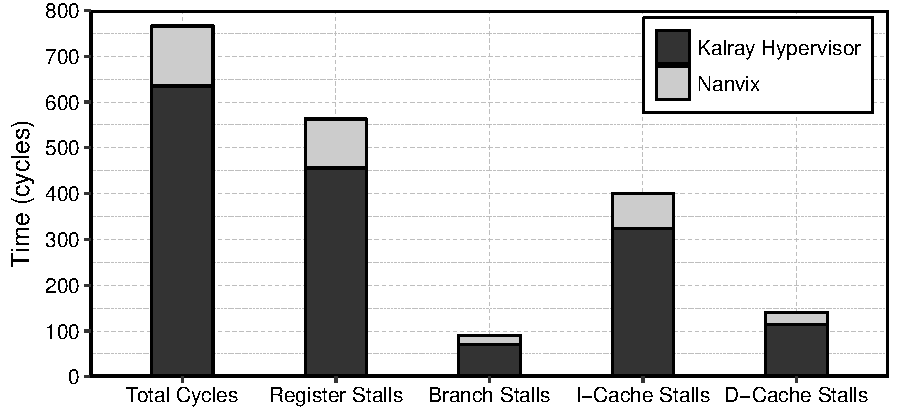
\includegraphics[width=1.00\linewidth]{ukernel-0a0088b/kcall-local-time-breakdown}
			\caption{Execution breakthrough for the \textit{\lkcall Benchmark}.}
			\label{fig:lkcall-result}
	\end{figure}

	\section{Trabalhos Correlatos}
\label{sec:related-work}

	ABC.

	\section{Conclusão}
\label{sec:conclusao}

	ABC.


	\bibliography{aux/references.bib}

\end{document}
